% !TEX root = ../../../report.tex

\FloatBarrier
\subsection{The FPGA Buses}\label{section:fpga-buses}

There are two buses in charge of communication with and on the FPGA. First, the
microcontroller communicates with the FPGA design using the External Bus
Interface (EBI) of the Giant Gecko microcontroller. Secondly, an internal bus is
used to transfer data to and from modules in the FPGA.

\subsubsection{The EBI Bus}
The EBI\cite{efm\_ebi} is a parallel bus with a separate data and address bus, in
addition to chip select, read-, and write-enable signals, all active low.

The communication between the MCU and the FPGA uses 23 address lines and 16 data
lines. All transfers are initiated when the chip select signal goes low. For
write transfers, the data and address lines are set up and the write enable
signal is asserted, see figure \ref{fig:ebi_write}.	

For reads, the address is set up and the data line is put in high impedance mode
before the read enable signal is asserted, see figure \ref{fig:ebi_read}.

\begin{figure}[h]
	\centering
	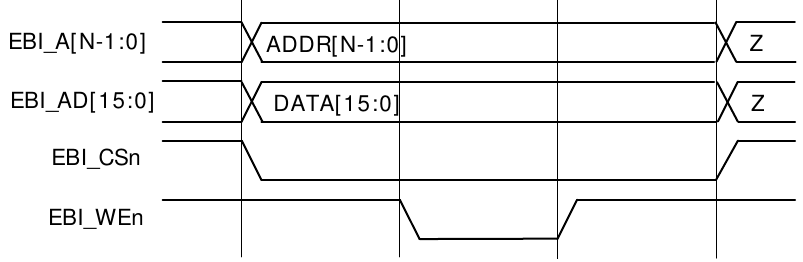
\includegraphics[width=0.8\linewidth]{figures/fpga/ebi_write.png}
	\caption{EBI write transfer\cite[p.6]{efm_ebi}}
	\label{fig:ebi_write}
\end{figure}



\begin{figure}[h]
	\centering
	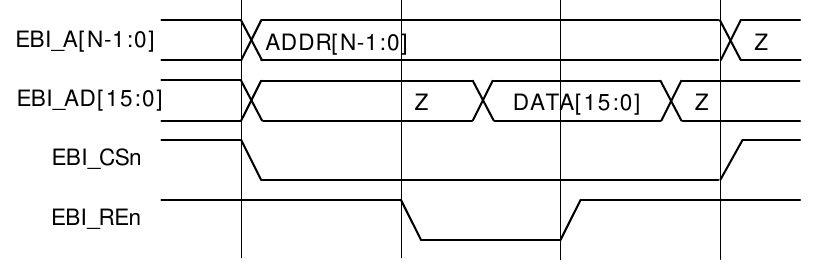
\includegraphics[width=0.8\linewidth]{figures/fpga/ebi_read.png}
	\caption{EBI read transfer\cite[p.7]{efm_ebi}}
	\label{fig:ebi_read}
\end{figure}



\FloatBarrier
\subsubsection{The Internal Bus}

All transfers are initiated by the microcontroller on the EBI bus, and the EBI
controller facilitates communication between the EBI and the internal bus.

\paragraph{The EBI controller}
The \textit{ebi\_controller} module is used to handle EBI transfers initiated by
the microcontroller. It consists of a simple state machine, illustrated in
figure \ref{fig:ebi_ctrl_fsm}. When an EBI transfer is executed, the internal
bus is used to store or load data from another module within the FPGA.

The \textit{ebi\_controller} keeps the EBI data lines in high impedance mode
whenever no transfer is active, allowing the MCU to have control of the EBI bus.

\begin{figure}[h]
	\centering
	% TODO: Make the arrows in separate directions be separate arrows
	\begin{tikzpicture}[shorten >= 1pt,node distance=2cm,on grid,auto]
		\node[state,initial] (idle) {idle};
		\node[state] (read) [above right=of idle] {read};
		\node[state] (write) [below right=of idle] {write};
		\path[->]
			(idle) edge node {\small RE = 0} (read)
			       edge node [swap] {\small EW = 0} (write)
			(read) edge node {\small RE = 1} (idle)
			(write) edge node [swap] {\small WE = 1} (idle);
	\end{tikzpicture}
	\caption{EBI controller state machine}
	\label{fig:ebi_ctrl_fsm}
\end{figure}




\FloatBarrier
\paragraph{Addressing}
\todo[inline]{Revise this ``addressing'' section and see if it should moved to
appendix.}

The input/output, control registers, and piplelines in the FPGA are addressed
using a simple addressing scheme, where the address is divided into several
parts, as illustrated in figure \ref{fig:ebi_addresses}.

\begin{figure}[H]
	\centering
	\begin{bytefield}[endianness=big,bitwidth=0.04\linewidth]{23}
		\bitheader{0-22}\\
		\bitbox{1}{T} &
		\bitbox{2}{\tiny Pipeline} &
		\bitbox{4}{Device} &
		\bitbox{2}{\tiny Subdev} &
		\bitbox{14}{Address}
	\end{bytefield}
	\caption{FPGA address format}
	\label{fig:ebi_addresses}
\end{figure}




In an EBI address, the T bit is used to select the toplevel control register.
If the T bit is set, the rest of the address is ignored, and only the toplevel
control register is accessible.

If the T bit is not set, the pipeline field is used to select which pipeline to
address. In a pipeline, the device field is used to select which module in the
pipeline to address.

\todo[inline]{Replace the below 0/1/2 digits with the more correct corresponding
hexadecimal adress value? (even if that means lots of padded zeroes. It makes it
tie better with what was just explained about the addressing.)}
Two device numbers have special meaning; device 0 is the pipeline control
register, while device 1 is the constant memory. All device numbers starting at
2 accesses the cores in the pipeline.

The subdevice field is used to select between modules in each core. These
subdevices are listed in table \ref{tab:core_subdevices}.

\begin{table}[h]
	\centering
	\begin{tabular}{|l l|}
		\hline
		\textbf{Number} & \textbf{Description} \\
		\hline
		0 & Control register \\
		1 & Instruction memory \\
		2 & Input buffer \\
		3 & Ouput buffer \\
		\hline
	\end{tabular}

	\caption{Processor core subdevices}
	\label{tab:core_subdevices}
\end{table}


\FloatBarrier
\paragraph{Read Transfers}

A read transfer is initiated when the read enable line from the microcontroller
goes active low. The EBI controller sets up the internal address signals and
asserts the internal read enable signal. This causes the requested data to be
available in the next clock cycle. The EBI controller switches to read state,
where it remains until the chip select signal is deasserted.

\paragraph{Write Transfers}

Write transfers are initiated the same way as read transfers. As the
write-enable signal goes low, the destination address is latched into the
internal address bus and the internal data lines are set to the value of the EBI
data lines. The EBI controller enters write state and the internal write enable
signal is asserted. The idle state is re-entered when the chip select is
deasserted.
